%%---------- Opzetten PoC----------\left( 
\chapter{Opzet Proof of Concept}
\label{ch:opzet-poc}
\section{Uit te werken scenario}\label{poc-scenario}
Het uit te werken scenario omvat vooral de hoofdfunctionaliteit van het Davo Group hun klantenportaal. Een gebruiker zal moeten kunnen inloggen en het verbruik van een telefoonnummer raadplegen. De data omvat het verbruik van mobiele telefoonnummers, zijnde datatype (sms, gesprek, bericht) en de hoeveelheid daarvan. In het verbruiksoverzicht zal het totale verbruik berekend worden, wat er voor zorgt dat er een resource intensieve functie aanwezig is. Zoals vermeldt in hoofdstuk \ref{sota-title-architecturen} is de invloed van zo een functie op de volledige applicatie verschillend per architectuur. Zo is bijvoorbeeld bij de microservice architectuur enkel de service waar die resource intensieve functie uitgevoerd wordt vertraagd terwijl de andere services hier geen of weinig hinder van ondervinden. 

\section{Bouwen applicatie}
\subsection{Ontwikkelomgeving}\label{poc-ontwikkelomgeving}
De applicaties worden ontwikkeld in PHP 8.3\footnote{https://www.php.net/} in combinatie met CodeIgniter 4\footnote{https://codeigniter.com/}. Dit is een server sided web frameworks binnen PHP die heel wat configuratie automatisch genereert voor een web applicatie. Ook security wordt standaard afgehandeld. De keuze van PHP werd gemaakt om in lijn te zijn met het klantenportaal van Davo Group, die ook op PHP draait en hetzelfde framework. Dit blijkt uit figuur \ref{verbruik_taal_sota}. De ontwikkeling gebeurt in de Visual Studio Code IDE\footnote{https://code.visualstudio.com/} en de applicatie wordt gehost op een lokale Apache\footnote{https://httpd.apache.org/} server. De applicatie wordt bijgehouden door het versiecontrolesysteem Github\footnote{https://github.com/} in de repository LuccaVanVeerdeghem/BachelorPOC\footnote{https://github.com/LuccaVanVeerdeghem/BachelorPOC}.


\subsection{Applicatie componenten}\label{oPOC_AC}
Alhoewel de structuur van iedere architectuur verschillend is, kan er toch een lijst opgesteld worden met de noodzakelijke componenten die nodig zijn om het scenario als applicatie op te stellen. Hieronder vallen database keuze, entiteiten, relaties, alsook controllers in de applicatie voor de entiteiten. Een controller is een klasse binnen de applicatie die methodes bevat om berekeningen uit te voeren met data die hij verkrijgt uit de database.\\

Voor de database wordt gewerkt met MySQL Community Server versie 8.0.27. De entiteiten die nodig zijn binnen deze database zijn Gebruiker, Telefoonnummer en Call Log. Een gebruiker kan meerdere telefoonnummers hebben, maar een telefoonnummer is gekoppeld aan één gebruiker. Een telefoonnummer kan meerdere call logs hebben, maar een call log is gekoppeld aan één telefoonnummer. Dit schema wordt voorgesteld in figuur \ref{bap_erd}.\\ 
\begin{figure}[h!]
    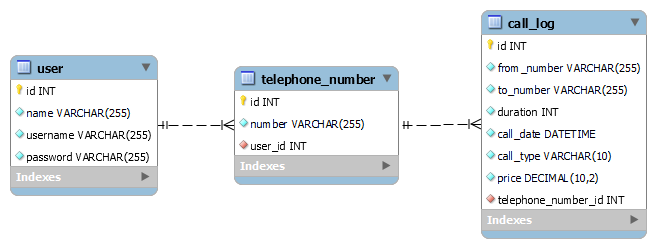
\includegraphics[scale=0.5]{bap_erd}
    \caption{ERD diagram PoC database}
    \label{bap_erd}
\end{figure}

De data die gebruikt wordt binnen deze PoC wordt gegenereerd door een MySQL script. Deze creëert eerst de database tabellen, gevolgd door het invullen van data voor de gebruikers en telefoonnummers. Zo worden er 3 gebruikers aangemaakt en 4 telefoonnummers. Eenmaal deze bestaan kan er door een algoritme, die opgeslagen wordt als een stored procedure, call logs gegenereerd worden. Er wordt eerst een random telefoonnummer geselecteerd uit de telefoonnummers tabel om te bepalen aan welk telefoonnummer de call log gekoppeld moet worden. Vervolgens wordt een bestemmingsnummer, log type (data, gesprek of sms), hoeveelheid, datum binnen 2 maand en prijs gegenereerd en ingevuld voor die specifieke call log. Dit doet hij 10000 keer, wat gemiddeld 2500 call logs per telefoonnummer voorziet. Het script is beschikbaar in bijlage \ref{bij_database}.\\ 


Aangezien de use case en entiteiten gekend zijn, kan er per controller ook een lijst van methodes en hun nut uitgeschreven worden. Voor de gebruiker controller moet er een login methode zijn die toegang verleent tot de applicatie, alsook een getUser om data te kunnen tonen van een gebruiker. De telefoonnummer controller heeft een getTelephoneNumber om de details ervan op te halen en een functie calculateUsage die het verbruik opvraagt aan de call log controller. Deze laatste controller beschikt dus ook over een calculateUsage methode, gevolgd door een getCallLogUsage die het verbruik van 1 call log ophaalt.\\ %todo aan te vullen met eventueel andere methodes. 

\subsection{Uitwerking methodes}
\subsubsection{Gebruiker}
De login methode laat gebruikers toe tot het dashboard indien er al een ingelogde sessie bestaat, anders toont deze de login pagina. Voor validatie van login pogingen wordt de validate\_login methode gebruikt. Door middel van een POST request wordt de gebruikersnaam en het wachtwoord doorgegeven aan de methode. Deze delegeert de login gegevens aan de gebruikersmodel, die de gebruiker ophaalt uit de database. Bij een succesvolle match wordt er een sessie gestart in PHP om de gebruiker bij te houden en volgt er een doorverwijzing naar de dashboardpagina. Bij een niet succesvolle inlogpoging wordt er teruggekeerd naar de login pagina en wordt er een error getoond. Als laatste bevat deze controller een logout functie, die de PHP sessie verwijdert en terugkeert naar de login pagina. De uitgewerkte controller en model zijn beschikbaar in bijlage \ref{bij_con_user} en \ref{bij_model_user}.\\


\subsubsection{Telefoonnummer}
Voor de telefoonnummer entiteit wordt enkel een overzicht opgehaald van telefoonnummers gekoppeld aan de ingelogde gebruiker. In de controller, op de index functie, wordt via de model de gekoppelde telefoonnummers opgehaald en weergegeven in de view. De uitgewerkte controller en model zijn beschikbaar in bijlage \ref{bij_con_telephone} en \ref{bij_model_telephone}.\\\\


\subsubsection{Call Log}
Als laatste blijft de Call Log over. De controller is verantwoordelijk voor het tonen van het verbruik van 1 telefoonnummer. Dit doet hij door via de model alle gelinkte logs op te vragen en vervolgens via een functie het verbruik te berekenen per groep, zijnde gesprek, sms en data. Door het overlopen van grote aantallen logs kan dit snel een resource intensieve methode worden. In het geval van deze proof of concept is dit gemiddeld 2500 logs per telefoonnummer, zoals eerder vermeldt in hoofdstuk \ref{oPOC_AC}. De uitgewerkte controller en model zijn beschikbaar in bijlage \ref{bij_con_calllog} en \ref{bij_model_calllog}.\\


\subsection{Monoliet}
De opbouw van de monoliet applicatie is vrij eenvoudig voor een doorsnee ontwikkelaar. Alles wordt verzameld binnen één applicatie en alle communicatie, zijnde gebruik van functies en methodes, kan intern gebeuren zonder hulp van API's. In de Proof of Concept wordt gebruik gemaakt van het MVC patroon, dat de database, business logica en user interface van elkaar afscheidt. De structuur van de applicatie wordt weergegeven in figuur \ref{monolith_structure}. \\

\begin{figure}[h!]
    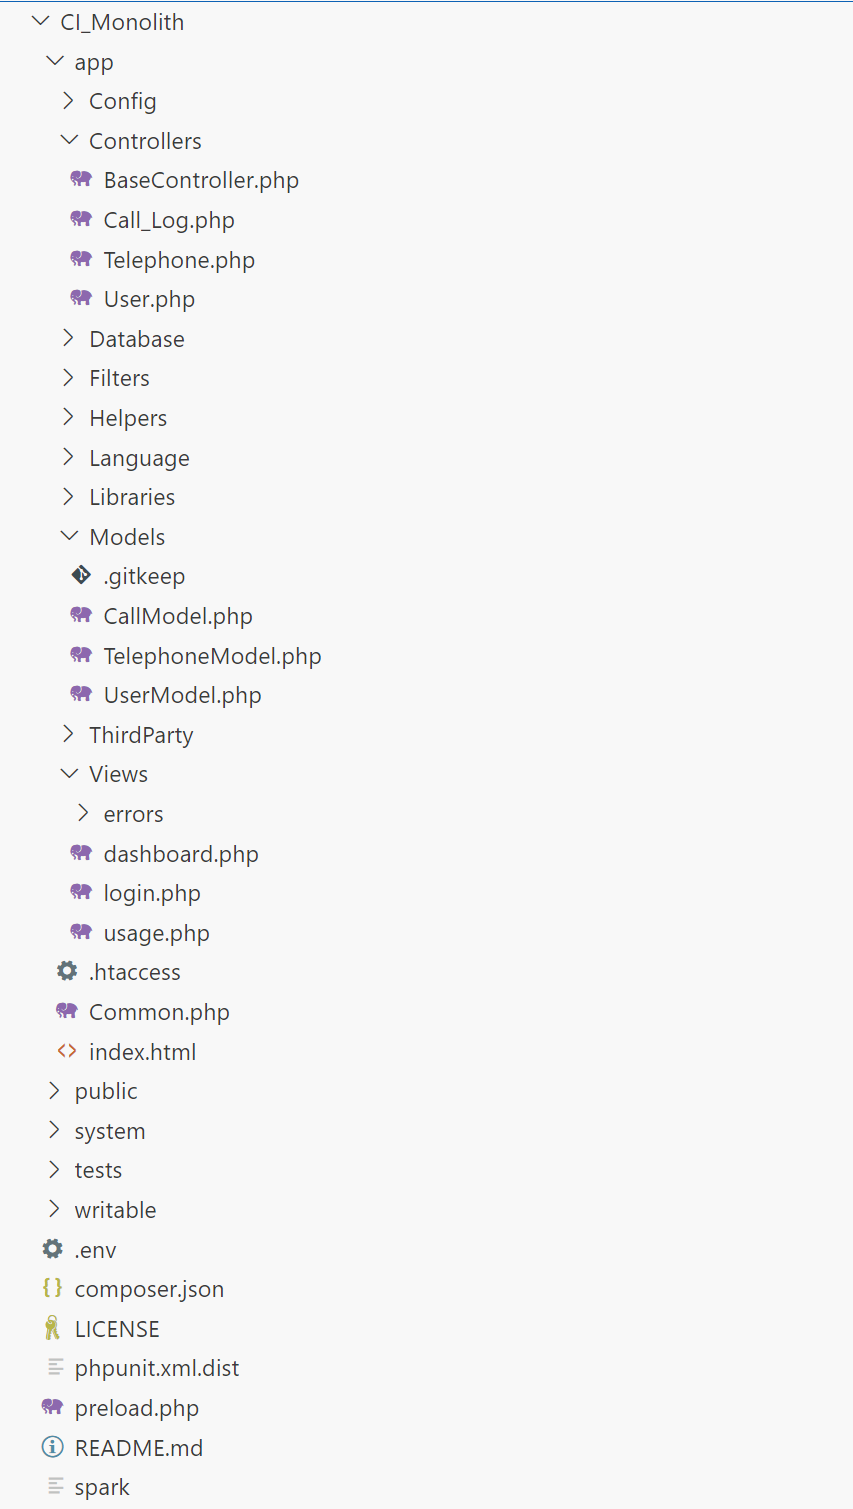
\includegraphics[scale=0.5]{monolith_structure}
    \caption{Applicatie structuur monoliet}
    \label{monolith_structure}
\end{figure}

\subsection{Microservice}
Een microservice applicatie zit net iets anders in elkaar dan een monoliet. Aangezien elke service zijn eigen 'applicatie' is, kan je stellen dat er meerdere 'monolieten' zijn die samenwerken om in zijn geheel als microservices te werken. En net omdat er meerdere applicaties zijn, is er ook nood aan een API, die niet nodig is bij de monoliet applicatie. Verder wordt de frontend afgehandeld met het BFF, backend for frontend, patroon. Dit design pattern zorgt ervoor dat eerst alle data van de backend, zijnde van de verschillende API's die gelinkt zijn aan hun eigen microservice, opgehaald is om dan te tonen op de webpagina. \\

De verschillende microservices worden voorgesteld in figuur \ref{multiple_microservices}. Er zijn 3 services die voor elke entiteit zijn functionaliteit afhandelen en één service die het BFF patroon uitvoert. De structuur van een service die een entiteit afhandelt wordt voorgesteld in figuur \ref{microservice_layout}. Hier valt op dat er een API controller is bijgekomen. Dit komt omdat elke microservice nu zijn data beschikbaar moet stellen via API, zodanig de service die de frontend toont alle data kan ophalen. De code van zo een API controller wordt voorgesteld in bijlage \ref{bij_api_con_call_log}. Hierin is het verschil tussen een gewone controller, zoals uit de monoliet applicatie, dat de data niet aan een view gegeven wordt maar als JSON wordt teruggegeven.\\

\begin{figure}[h!]
    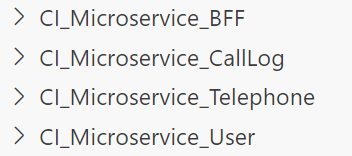
\includegraphics{microservice_structure}
    \caption{Verschillende microservices}
    \label{multiple_microservices}
\end{figure}

\begin{figure}[h!]
    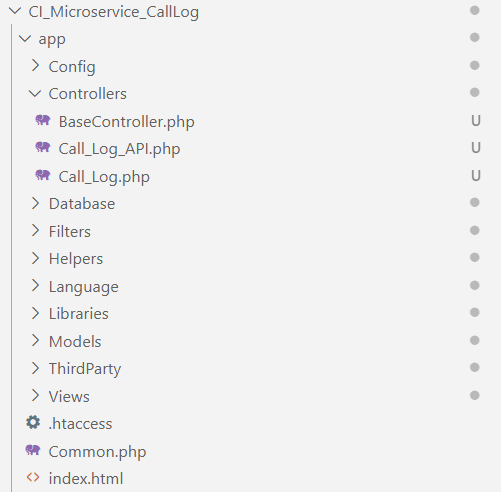
\includegraphics[scale=0.75]{microservice_layout}
    \caption{Structuur van een microservice}
    \label{microservice_layout}
\end{figure}

De structuur van de BFF service is terug te vinden in figuur \ref{microservice_bff_layout}. Voor elke entiteit is hier een controller te vinden, zoals bij de monoliet applicatie. Echter is hier nog altijd een verschil, aangezien de BFF service zelf geen toegang heeft tot data. Daarvoor maakt deze gebruik van curl, een ingebouwde functie om HTTP requests te versturen, om data op te halen van elke service wanneer hij die data nodig heeft. Een voorbeeld hiervan is terug te vinden in bijlage \ref{bij_ms_con_call_log}.\\

\begin{figure}[h!]
    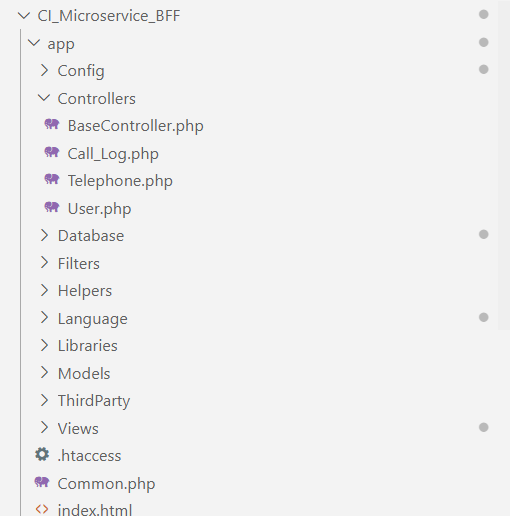
\includegraphics[scale=0.75]{microservice_bff_layout}
    \caption{Structuur van BFF patroon microservice}
    \label{microservice_bff_layout}
\end{figure}

\subsection{Opzetten testomgeving}
Als testomgeving zal er voor de monoliet een Apache server op een Ubuntu Desktop 24.04 LTS\footnote{https://ubuntu.com/}. De keuze voor een Linux systeem ligt bij de mogelijkheden om per proces het energieverbruik te kunnen meten. Voor de microservices wordt er gebruik gemaakt van Docker\footnote{https://www.docker.com/} om de services individueel te laten draaien. De configuratie van de docker-compose omgeving is terug te vinden in bijlage \ref{bij_docker}. Deze maakt 4 verschillende Apache servers aan, 1 voor elke service die later besproken worden, en 1 MySQL server\footnote{https://www.mysql.com/}. Door het uitvoeren van het commando \textit{(sudo) docker-compose up} in de root folder van de PoC komen deze services actief en is de gebruikers interface bereikbaar op http://localhost:8081/public/.\\

Voor het meten van energieverbruik per applicatie is gebruik gemaakt van PowerJoular. Deze software is geschreven in Ada\footnote{https://ada-lang.io/} kan gecompileerd worden door een GNAT compiler\footnote{https://www.gnu.org/software/gnat/}. Voor de installatie van alle gebruikte software binnen de testomgeving is een installatiescript voorzien, deze is beschikbaar in bijlage \ref{bij_installatie_software}.// %todo script instellen

De relevante hardware configuratie van de machine bestaat als volgt:
\begin{itemize}
    \item Aorus B450 moederbord;
    \item AMD Ryzen 7 5900 CPU;
    \item 48GB DDR4 3200Mhz RAM;
    \item Gigabyte RTX 2070 OC 8GB GPU.
\end{itemize}